%\pagestyle{codienhiendai}
\pagestyle{codienhiendai}
\thispagestyle{codienhiendainone}
\graphicspath{{../codienhiendai/pic/}}
%\blfootnote{$^1$Department of Mathematics, The University of Akron, Akron,
%	Ohio $44325$, USA}
\begingroup
\AddToShipoutPicture*{\put(0,0){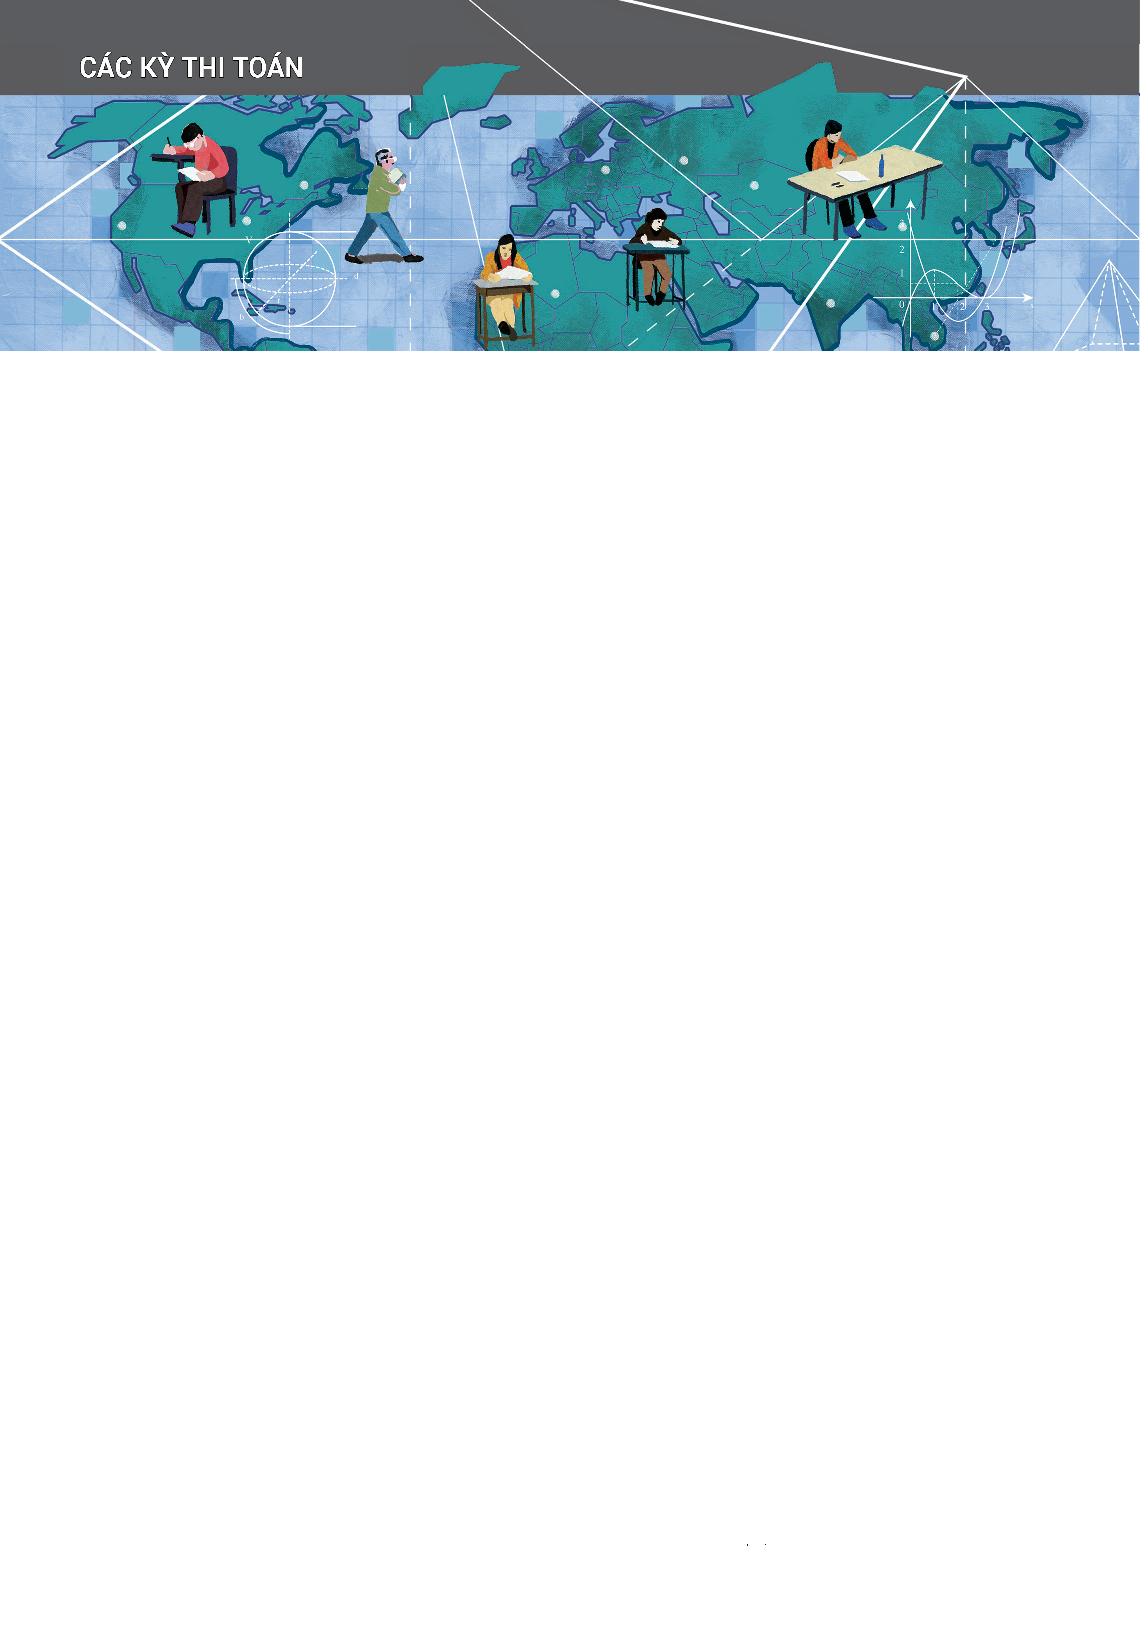
\includegraphics[scale=1]{../banner.pdf}}}
\AddToShipoutPicture*{\put(80,490){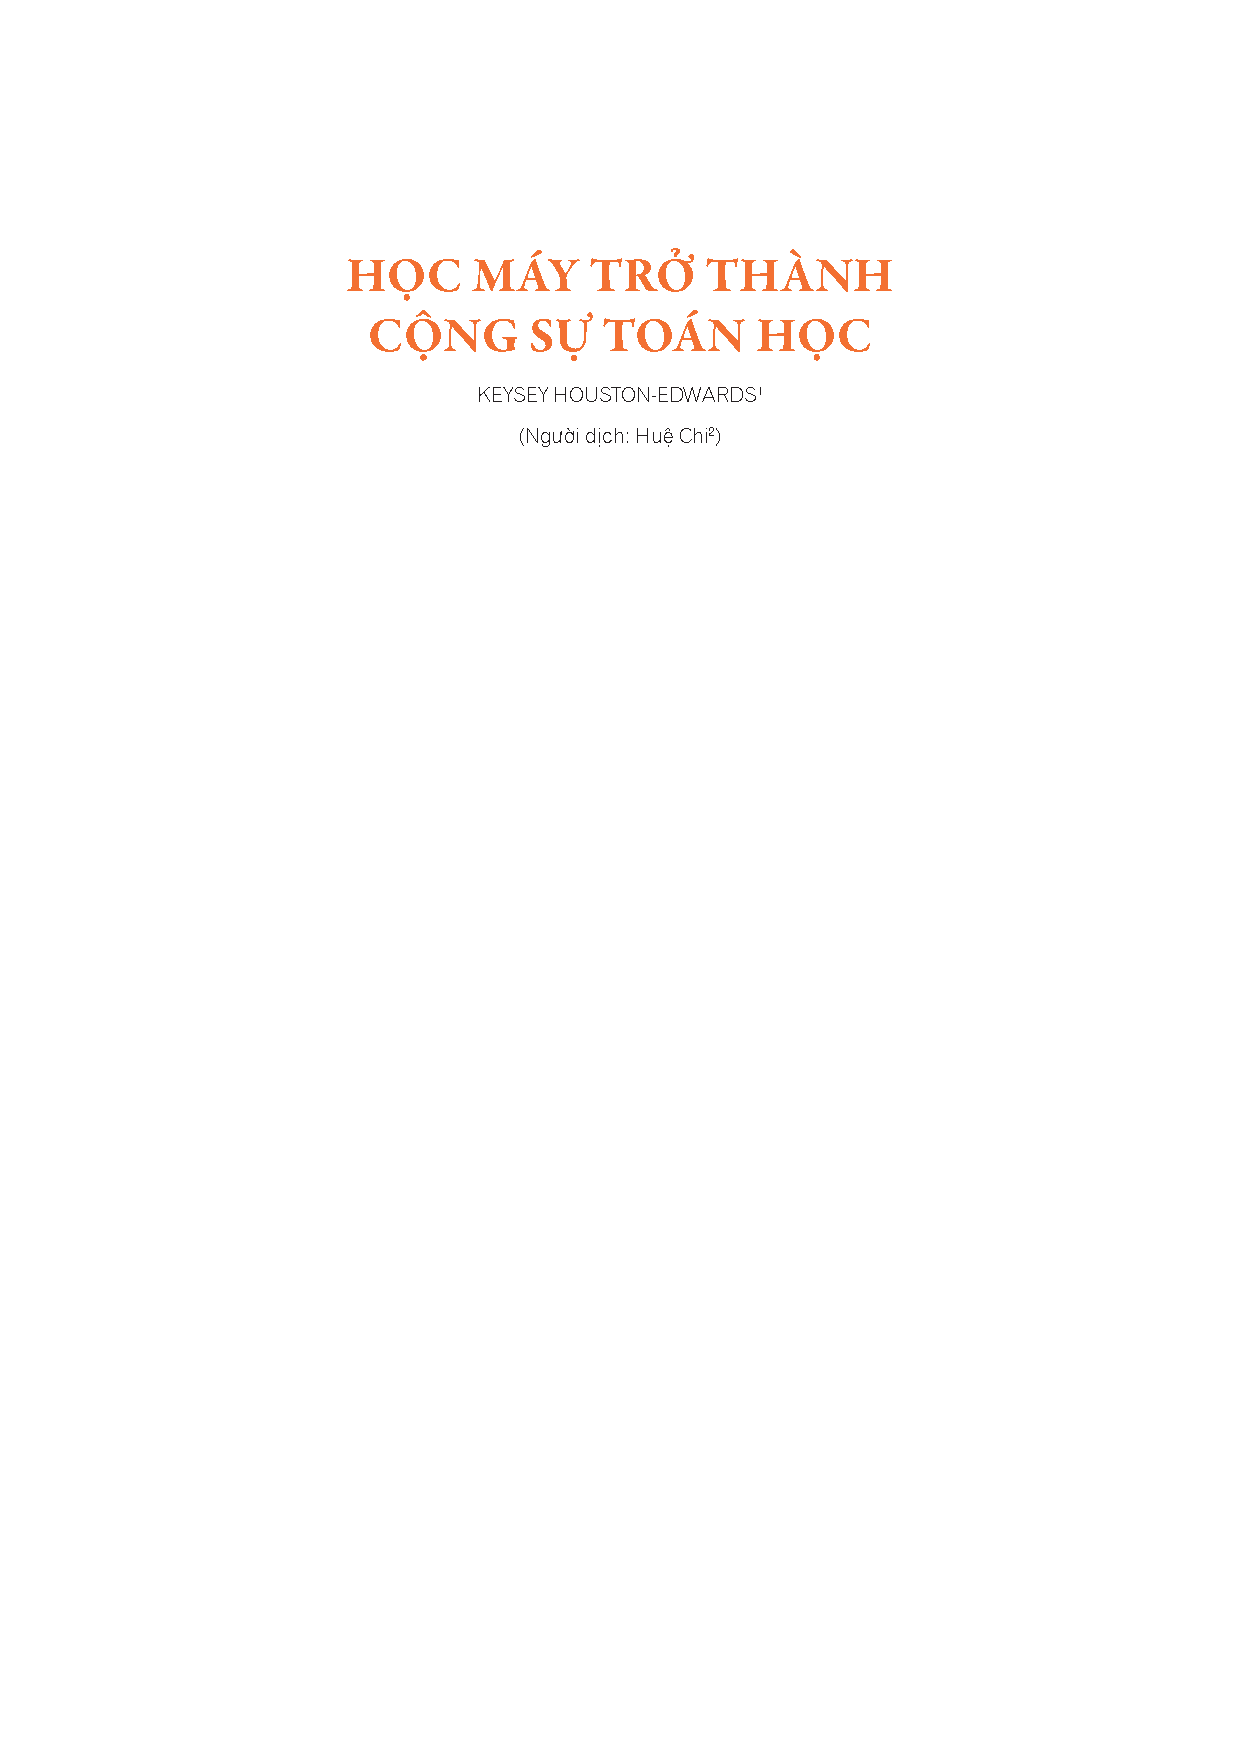
\includegraphics[scale=1]{../tieude1.pdf}}} 
\centering
\endgroup

\vspace*{220pt}
\begin{multicols}{2}
	Ngày $24$ tháng $7$ năm $2017$
	\vskip 0.1cm
	\textit{Sau khi qua đời khi còn rất trẻ, cuộc đời của Maryam Mirzakhani được {\color[named]{codienhiendai}ghi nhớ một cách} trọn vẹn nhất qua các công trình của cô ấy.}
	\begin{figure}[H]
		\centering
		\vspace*{-5pt}
		\captionsetup{labelformat= empty, justification=centering}
		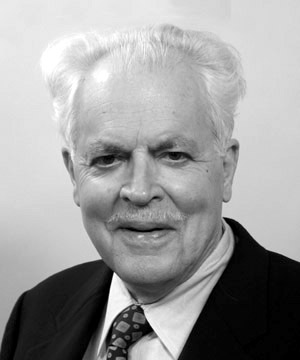
\includegraphics[width=0.475\textwidth]{2}
		\caption{\small\textit{{\color[named]{codienhiendai}Maryam Mirzakhani năm $2014$.}}}
		\vspace*{-10pt}
	\end{figure}
	Những day dứt của sự buồn bã ập đến sau những tin tức về {\color[named]{codienhiendai}cái chết} của Maryam \linebreak Mirzakhani đã thôi thúc tôi đọc tất cả những bài báo viết về cô ấy mà tôi tìm được, và khi không thể tìm thêm những bài báo khác, tôi bắt đầu đọc những bình luận của độc giả. Nhiều người trong số họ đã viết rằng họ cảm thấy cô ấy thật ``xa lạ và khó hiểu" y như những bài toán hóc búa. Tuy nhiên, Maryam không hề xa lạ. Bằng lời nói và hành động, cô ấy đã cho chúng ta thấy rằng những ý tưởng toán học đêù có thể thấu hiểu được nếu như người ta có đủ kiên trì để tìm hiểu chúng.
	\vskip 0.1cm
	Cô ấy không phải là ngôi sao trong các bài giảng của mình, những ý tưởng toán học là những ngôi sao duy nhất. Cô ấy giảng bài một cách điềm tĩnh, rõ ràng và {\color[named]{codienhiendai}toả ra một nỗi} hứng thú {\color[named]{codienhiendai}sâu sắc} với công việc đó. 
	\vskip 0.1cm
	Cô ấy có khả năng nhanh chóng bắt được {\color[named]{codienhiendai}bước} sóng {\color[named]{codienhiendai}tương ứng} của người đối thoại và biết cách nói chuyện sao cho phù hợp, một phẩm chất hiếm có ở một nhà toán học. Cô ấy lắng nghe chăm chú và rất thoải mái về mặt thời gian. Đằng sau sự {\color[named]{codienhiendai}điềm tĩnh} dịu dàng của cô ấy người ta có thể nhận thấy một sự bền bỉ cứng như thép và một kho ý tưởng sâu sắc, và tất nhiên là một sự say mê toán học và một cuộc tìm kiếm không ngừng nghỉ cho một khoảnh khắc bùng nổ tuyệt vời. Khoảnh khắc này thường khiến cô ấy mất vài năm, bởi vì cô ấy nghiên cứu những vấn đề uyên thâm.
	\vskip 0.1cm
	Một lần, sau bài giảng của cô ấy, chúng tôi đã cùng nhau trao đổi. Đột nhiên, tiếng của một đứa trẻ từ căn phòng kế bên vọng ra và Maryam đã quát lên ``Anahita!". Thì ra đó là tiếng của con gái cô ấy. Tiếng quát của \linebreak Maryam vang khắp căn phòng. Giọng cô ấy luôn khác hẳn khi giảng bài. Toàn bộ {\color[named]{codienhiendai}khía cạnh con người} của cô ấy đã thể hiện trong tiếng quát đó.
	\vskip 0.1cm
	Các công trình của Maryam đã kết nối các ý tưởng của nhiều lĩnh vực khác nhau của toán học. Một phần của những công trình này là việc đếm các đường cong đóng trên các  mặt. Một mặt trong toán học nói một cách nôm na là lớp ngoài cùng của một vật rắn. Trong topo, các mặt được nghiên cứu qua phép biến dạng, Chúng có thể được uốn cong, {\color[named]{codienhiendai}kéo giãn} nhưng không thể xé rách, giống như {\color[named]{codienhiendai}một câu đùa từ xưa nói} rằng nhà tôpô học không thể tạo được một tách cà phê từ một chiếc bánh donut. Các mặt cũng có các lỗ và các cạnh. Như vậy, một đĩa và một mặt trụ cũng có thể xem như các mặt. 
	\vskip 0.1cm
	Các đường cong đóng trên một mặt giống như những dây cao su cực kỳ mỏng bao \linebreak quanh nó. Các đường cong cũng được nghiên cứu qua phép biến dạng trên mặt. Chẳng hạn như, trên một mặt trụ, mỗi đường cong đóng có thể được biến dạng \linebreak thành một đường cong khác chạy quanh mặt trụ một lần, hai lần, ba lần hoặc nhiều hơn hoặc là không lần nào cả, tức là nó có thể biến dạng thành một điểm.
	\vskip 0.1cm
	Các mặt cũng có thể được nghiên cứu theo quan điểm hình học. Trong trường hợp này, một mặt nới rộng được có thể được bổ sung một metric--một cách để đo các khoảng cách và các góc.
	\vskip 0.1cm
	Các nhà toán học gọi mặt được xác định bởi lớp ngoài của một chiếc bánh donut là một xuyến. Một cách để xác định metric trên một xuyến là tưởng tượng chúng ta là những \linebreak sinh vật nhỏ bé đang sống trên bề mặt đa dạng của một chiếc bánh donut, nơi chúng ta đo các khoảng cách và các góc. Khung cảnh mà chúng ta nhìn thấy sẽ thay đổi khi chúng ta di chuyển từ nơi này sang nơi khác. 
	\vskip 0.1cm
	Có một cách khác để {\color[named]{codienhiendai}tiếp nhận được khái niệm}  một metric trên một xuyến, đó là tưởng tượng chúng ta vẫn là những sinh vật nhỏ bé nhưng đang sống trên một cái gì đó giống như hình vuông. Một `` cái gì đó" có một \linebreak tính chất đặc biệt sau: Nếu chúng ta đi theo một đường thẳng và {\color[named]{codienhiendai}chạm} đến một trong các \linebreak cạnh, chẳng hạn như cạnh phía trên, nếu chúng ta muốn tiếp tục đi thẳng thì chúng ta phải ``vào lại" từ cạnh phía dưới, đi theo hướng cũ và tại điểm ở ngay dưới điểm chúng ta đã đi ra. Một số trò chơi điện tử, như Pac--Man, diễn ra ở một hành tinh giống hình vuông như thế.
	\begin{figure}[H]
		\centering
		\vspace*{-5pt}
		\captionsetup{labelformat= empty, justification=centering}
		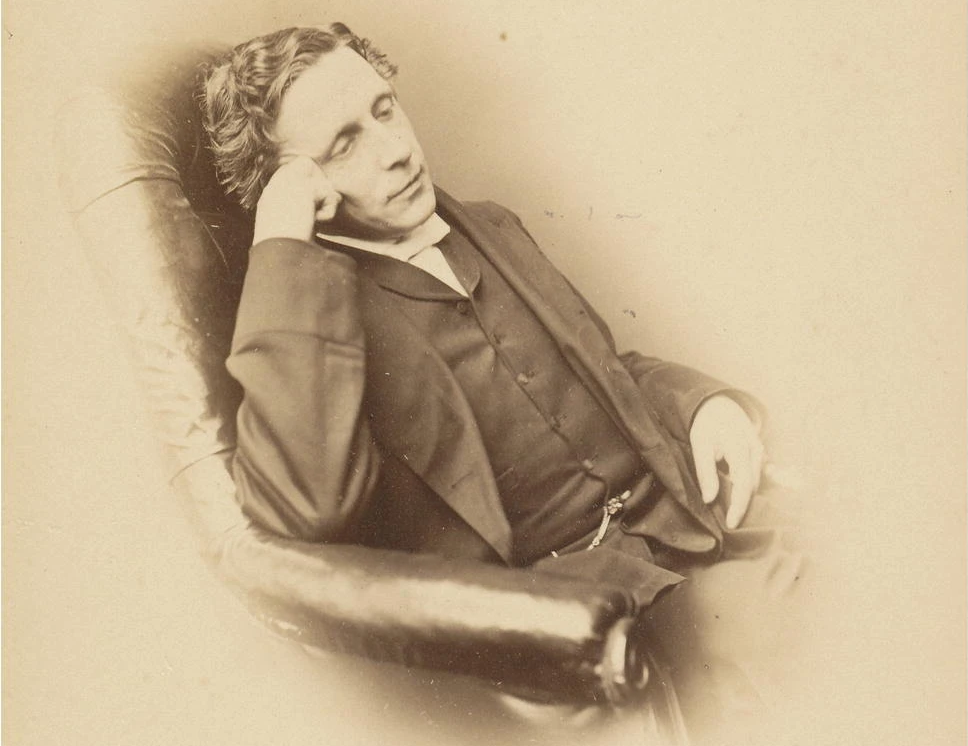
\includegraphics[width=0.475\textwidth]{1}
		\caption{\small\textit{{\color[named]{codienhiendai}Moira Chas là một nhà toán học tại đại học Stony Brook.}}}
		\vspace*{-10pt}
	\end{figure}
	Chúng ta cần suy nghĩ một chút để {\color[named]{codienhiendai}tự thuyết phục được} rằng hành tinh này cũng là một xuyến. Metric trong trường hợp này không phải là thứ mà chúng ta ``nhìn thấy" khi chúng ta sống trên bề mặt của một chiếc \linebreak bánh donut, nhưng ý tưởng về một cái gì đó giống hình vuông cho ta thấy ta có thể xác \linebreak định nó như thế nào. Một tính chất thú vị của metric Pac--Man là tại mọi điểm phong cảnh xung quanh chúng ta trông đều giống nhau. Nó hoàn toàn bằng phẳng.
	\vskip 0.1cm
	Nếu topo của một mặt ``đủ phức tạp" ( tức là, nó không phải là mặt cầu, xuyến, đĩa hay mặt trụ ), nó có thể được trang bị các \linebreak metric được gọi là metric hyperbolic. Trong các metric này, phong cảnh tại mỗi điểm trông giống như đèo  hoặc  khoai tây chiên Pringles. Giống như metric Pac--Man, những metric này không thể được hình dung như những khoảng cách đo được trên lớp ngoài cùng của bánh donut. Nhưng như chúng ta đã học được từ nhà toán học quá cố William Thurston, sau khi suy luận một chút, chúng ta có thể xem xét chúng từ góc độ toán học.
	\vskip 0.1cm
	Tập hợp tất cả những đường cong giống như những sợi dây cao su trên một mặt có thể biến dạng thành một đường cong cho trước được gọi là một lớp biến dạng. Một tính chất đáng chú ý của các metric hyperbolic là trong mỗi lớp biến dạng chỉ có một đường cong đóng có độ dài nhỏ nhất có thể. Đường cong ngắn nhất này được gọi là một đường \linebreak trắc địa.
	\vskip 0.1cm
	Một phần công việc của Maryam có liên quan đến việc đếm những đường trắc địa này trên các mặt với metric hyperbolic. Trước cô ấy, các nhà toán học đã biết rằng một mặt chỉ có hữu hạn các đường trắc địa với độ dài cố \linebreak định. Hơn nữa, các nhà toán học đã biết rằng số các đường trắc địa ngắn hơn một độ dài cho trước  tăng theo hàm mũ so với độ lớn của độ dài này. Tốc độ tăng như  hàm mũ này cản trở chúng ta thực hiện các tính toán \linebreak khảo sát.
	\vskip 0.1cm
	Một trong những bài toán mà Maryam đã giải đáp được là về tốc độ tăng của số các đường trắc địa không tự cắt. Cô ấy đã chia các đường trắc địa không tự cắt thành các loại. Hai đường trắc địa không tự cắt được xem là thuộc cùng một loại nếu chúng ``toạ lạc" trên một mặt theo cách thức tương đương nhau.
	\vskip 0.1cm
	Cô ấy đã chứng minh rằng trên một mặt \linebreak hyperbolic, số các đường trắc địa không tự cắt thuộc cùng một loại cho trước {\color[named]{codienhiendai}tăng theo độ} đa thức (không phải như hàm mũ) {\color[named]{codienhiendai}theo độ} tăng của độ dài. Điều này giúp cho các \linebreak tính toán khảo sát {\color[named]{codienhiendai}toàn diện}. Cô ấy đã đưa ra các công thức tường minh và có ý nghĩa cho các hệ số của đa thức này. (Độc giả có thể vẽ các đường cong đóng trên một mẩu giấy với ba lỗ thủng trên đó để bước đầu nhìn thấy độ phức tạp có thể có của các đường cong này.) Hơn nữa, công trình này đưa đến một chứng minh nguyên bản cho giả thuyết nổi tiếng của Edward Witten trong lý thuyết {\color[named]{codienhiendai}dây}.
	\vskip 0.1cm
	Cách đây {\color[named]{codienhiendai}chừng} hơn một thập kỷ một chút, khi cộng đồng toán học bắt đầu biết về \linebreak Maryam Mirzakhani, lúc đó {\color[named]{codienhiendai}từng thật} khó để phát âm đúng tên của cô ấy-- một cái tên {\color[named]{codienhiendai}khá} lạ. Sức mạnh và vẻ đẹp của các công trình của cô ấy đã thôi thúc chúng ta tập phát âm đúng tên cô. Thật đau lòng khi không còn Maryam ở bên {\color[named]{codienhiendai}cạnh} chúng ta. Cũng thật khó tin: sức mạnh của trí tuệ của cô ấy đã khiến tôi cảm thấy rằng đáng lẽ ra cô ấy có thể {\color[named]{codienhiendai}được che tránh} khỏi cái chết.
	\vskip 0.1cm
	Có lẽ cách tốt nhất để chúng ta tôn vinh và tưởng nhớ Maryam là tiếp tục phát triển những thành tựu tuyệt đẹp của cô ấy.
	\vskip 0.1cm
	\hfill Moira Chas
	\vskip 0.1cm
	\hfill $24$ tháng $7$ năm $2017$
\end{multicols}



